\section{Evaluation}
\label{sec:evaluation}

%In this section, we present the experimental settings, and the two experiments,
%based on synthetic and real-world datasets, that we used to assess our methodology.


\begin{figure*}[t]
    \centering
    \subfloat[\centering Definition of Deterministic BPSP with $q_U$\label{fig:calendar_qU}]{{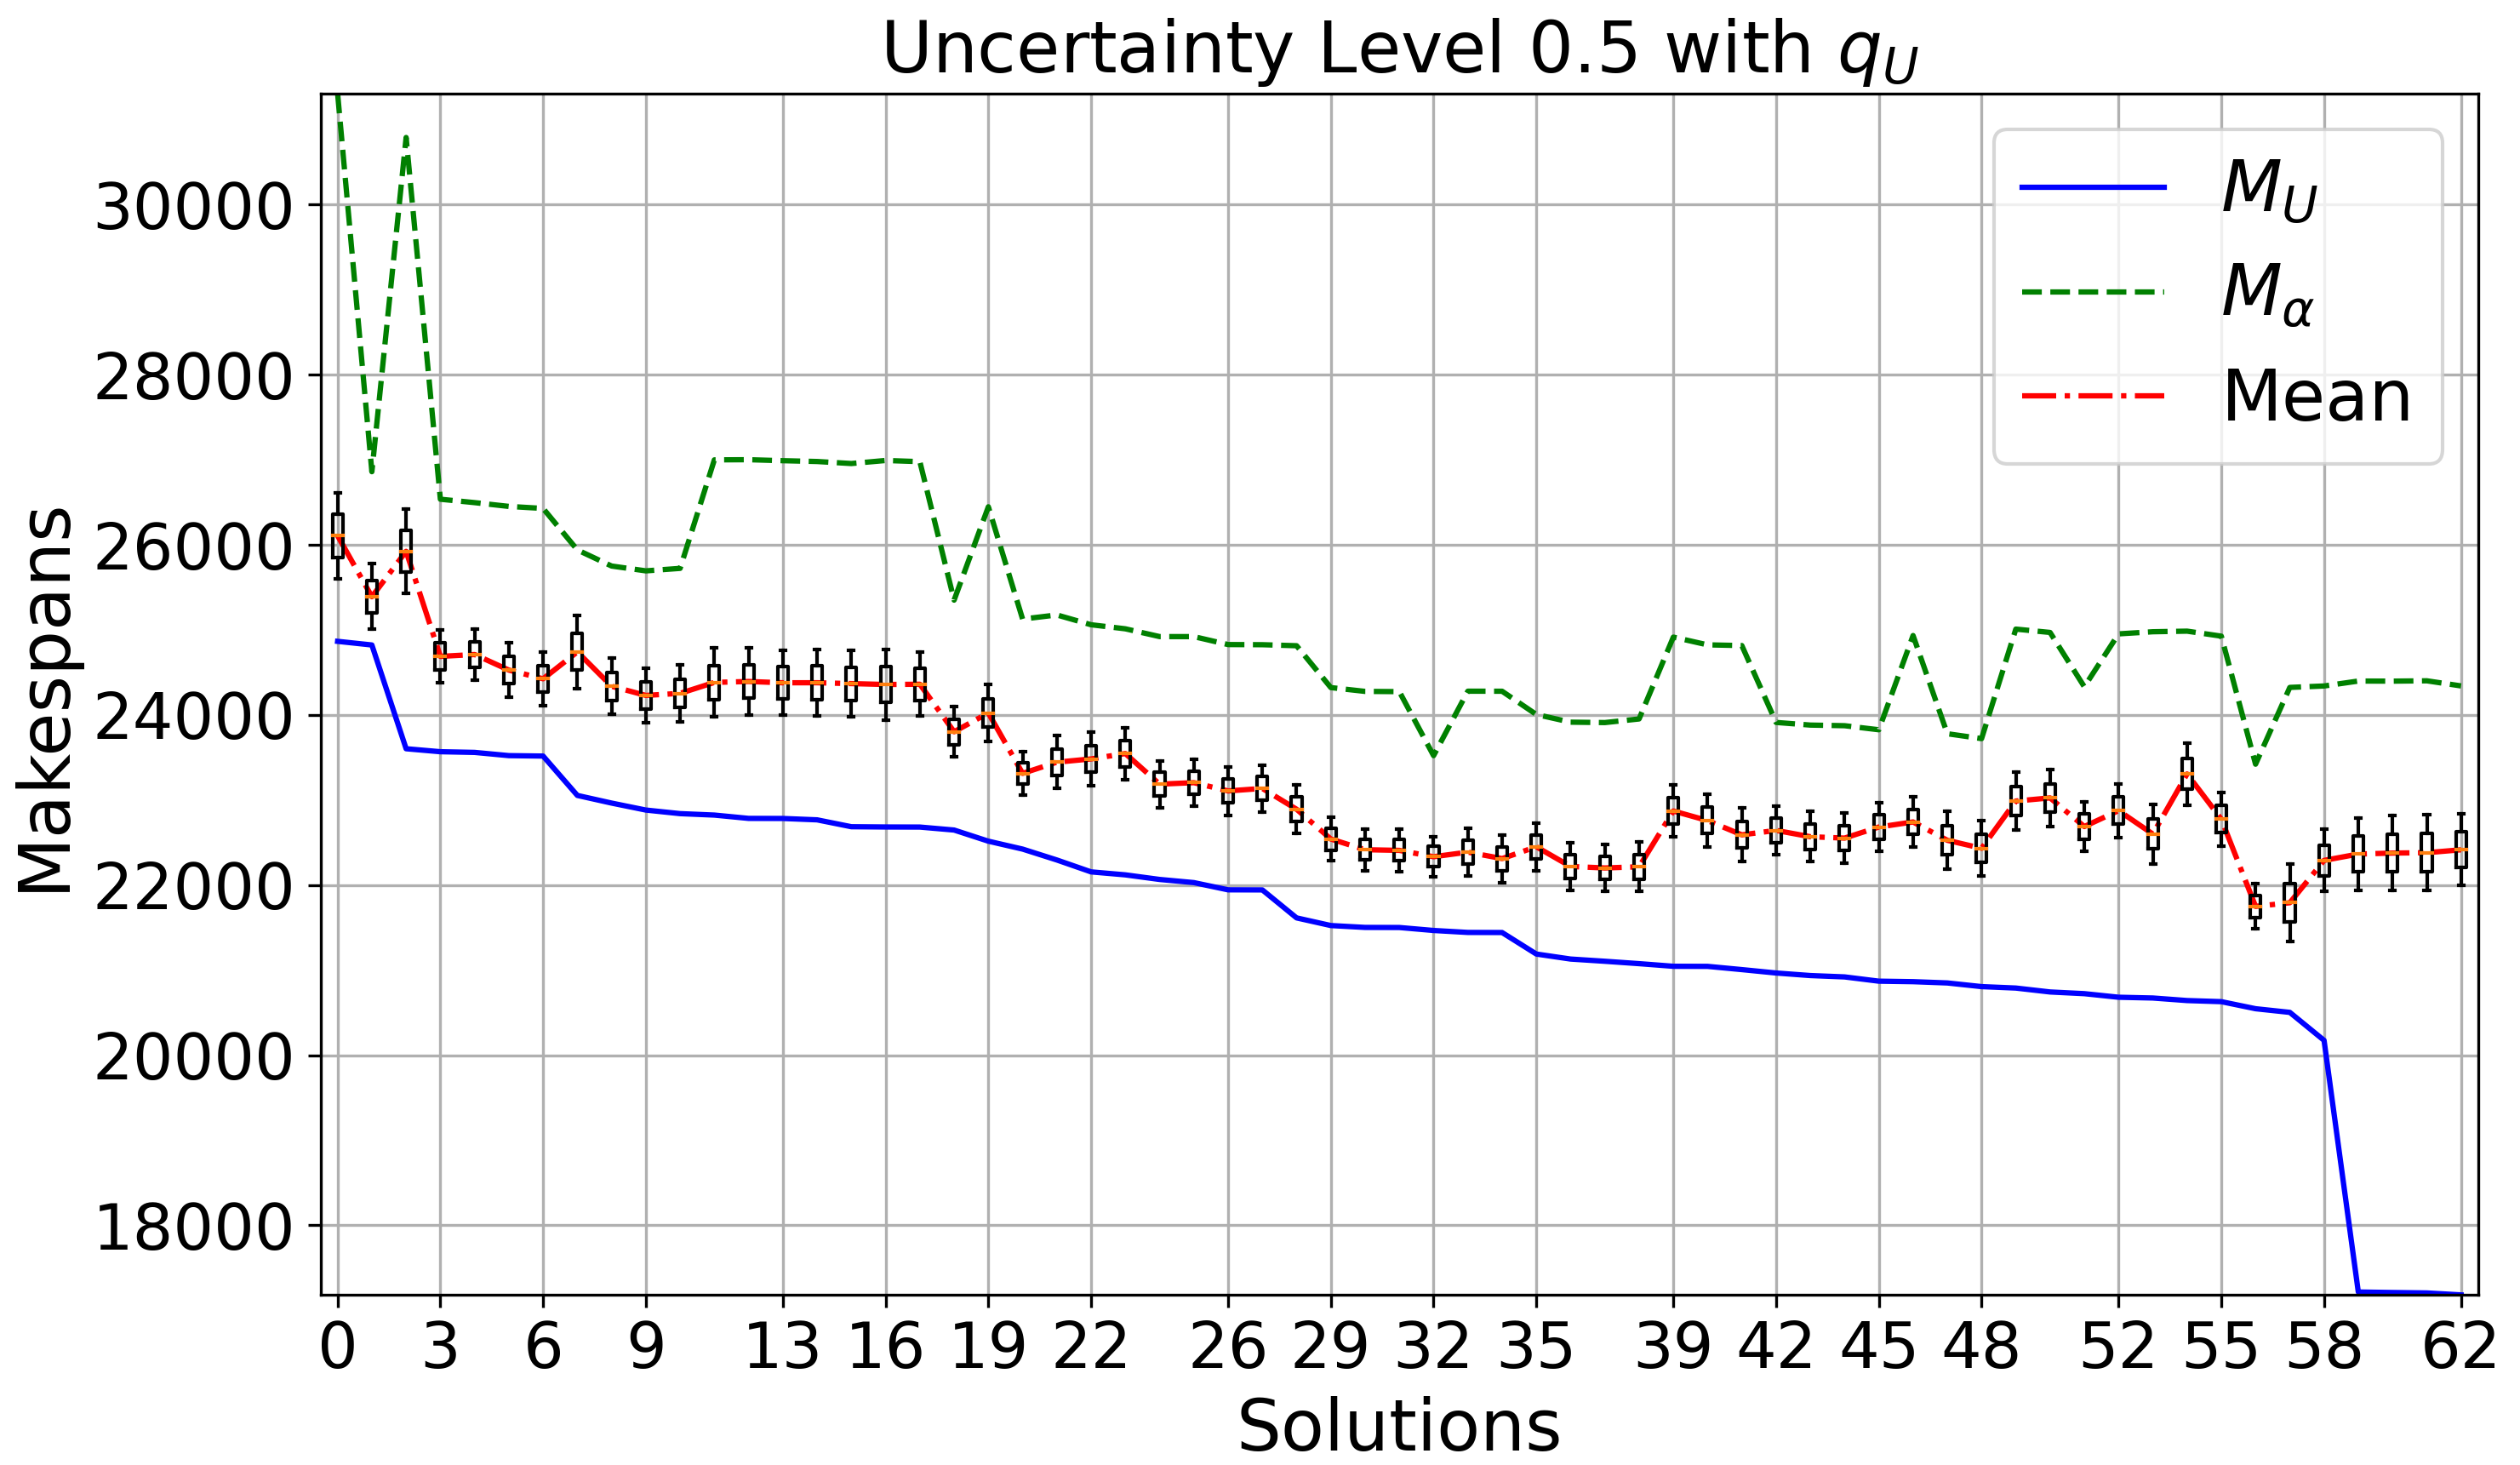
\includegraphics[width=0.47\textwidth]{images/uncertainty_caledars_1.png} }}%
    \qquad
    \subfloat[\centering Definition of Deterministic BPSP with $q_C$\label{fig:calendar_qC}]{{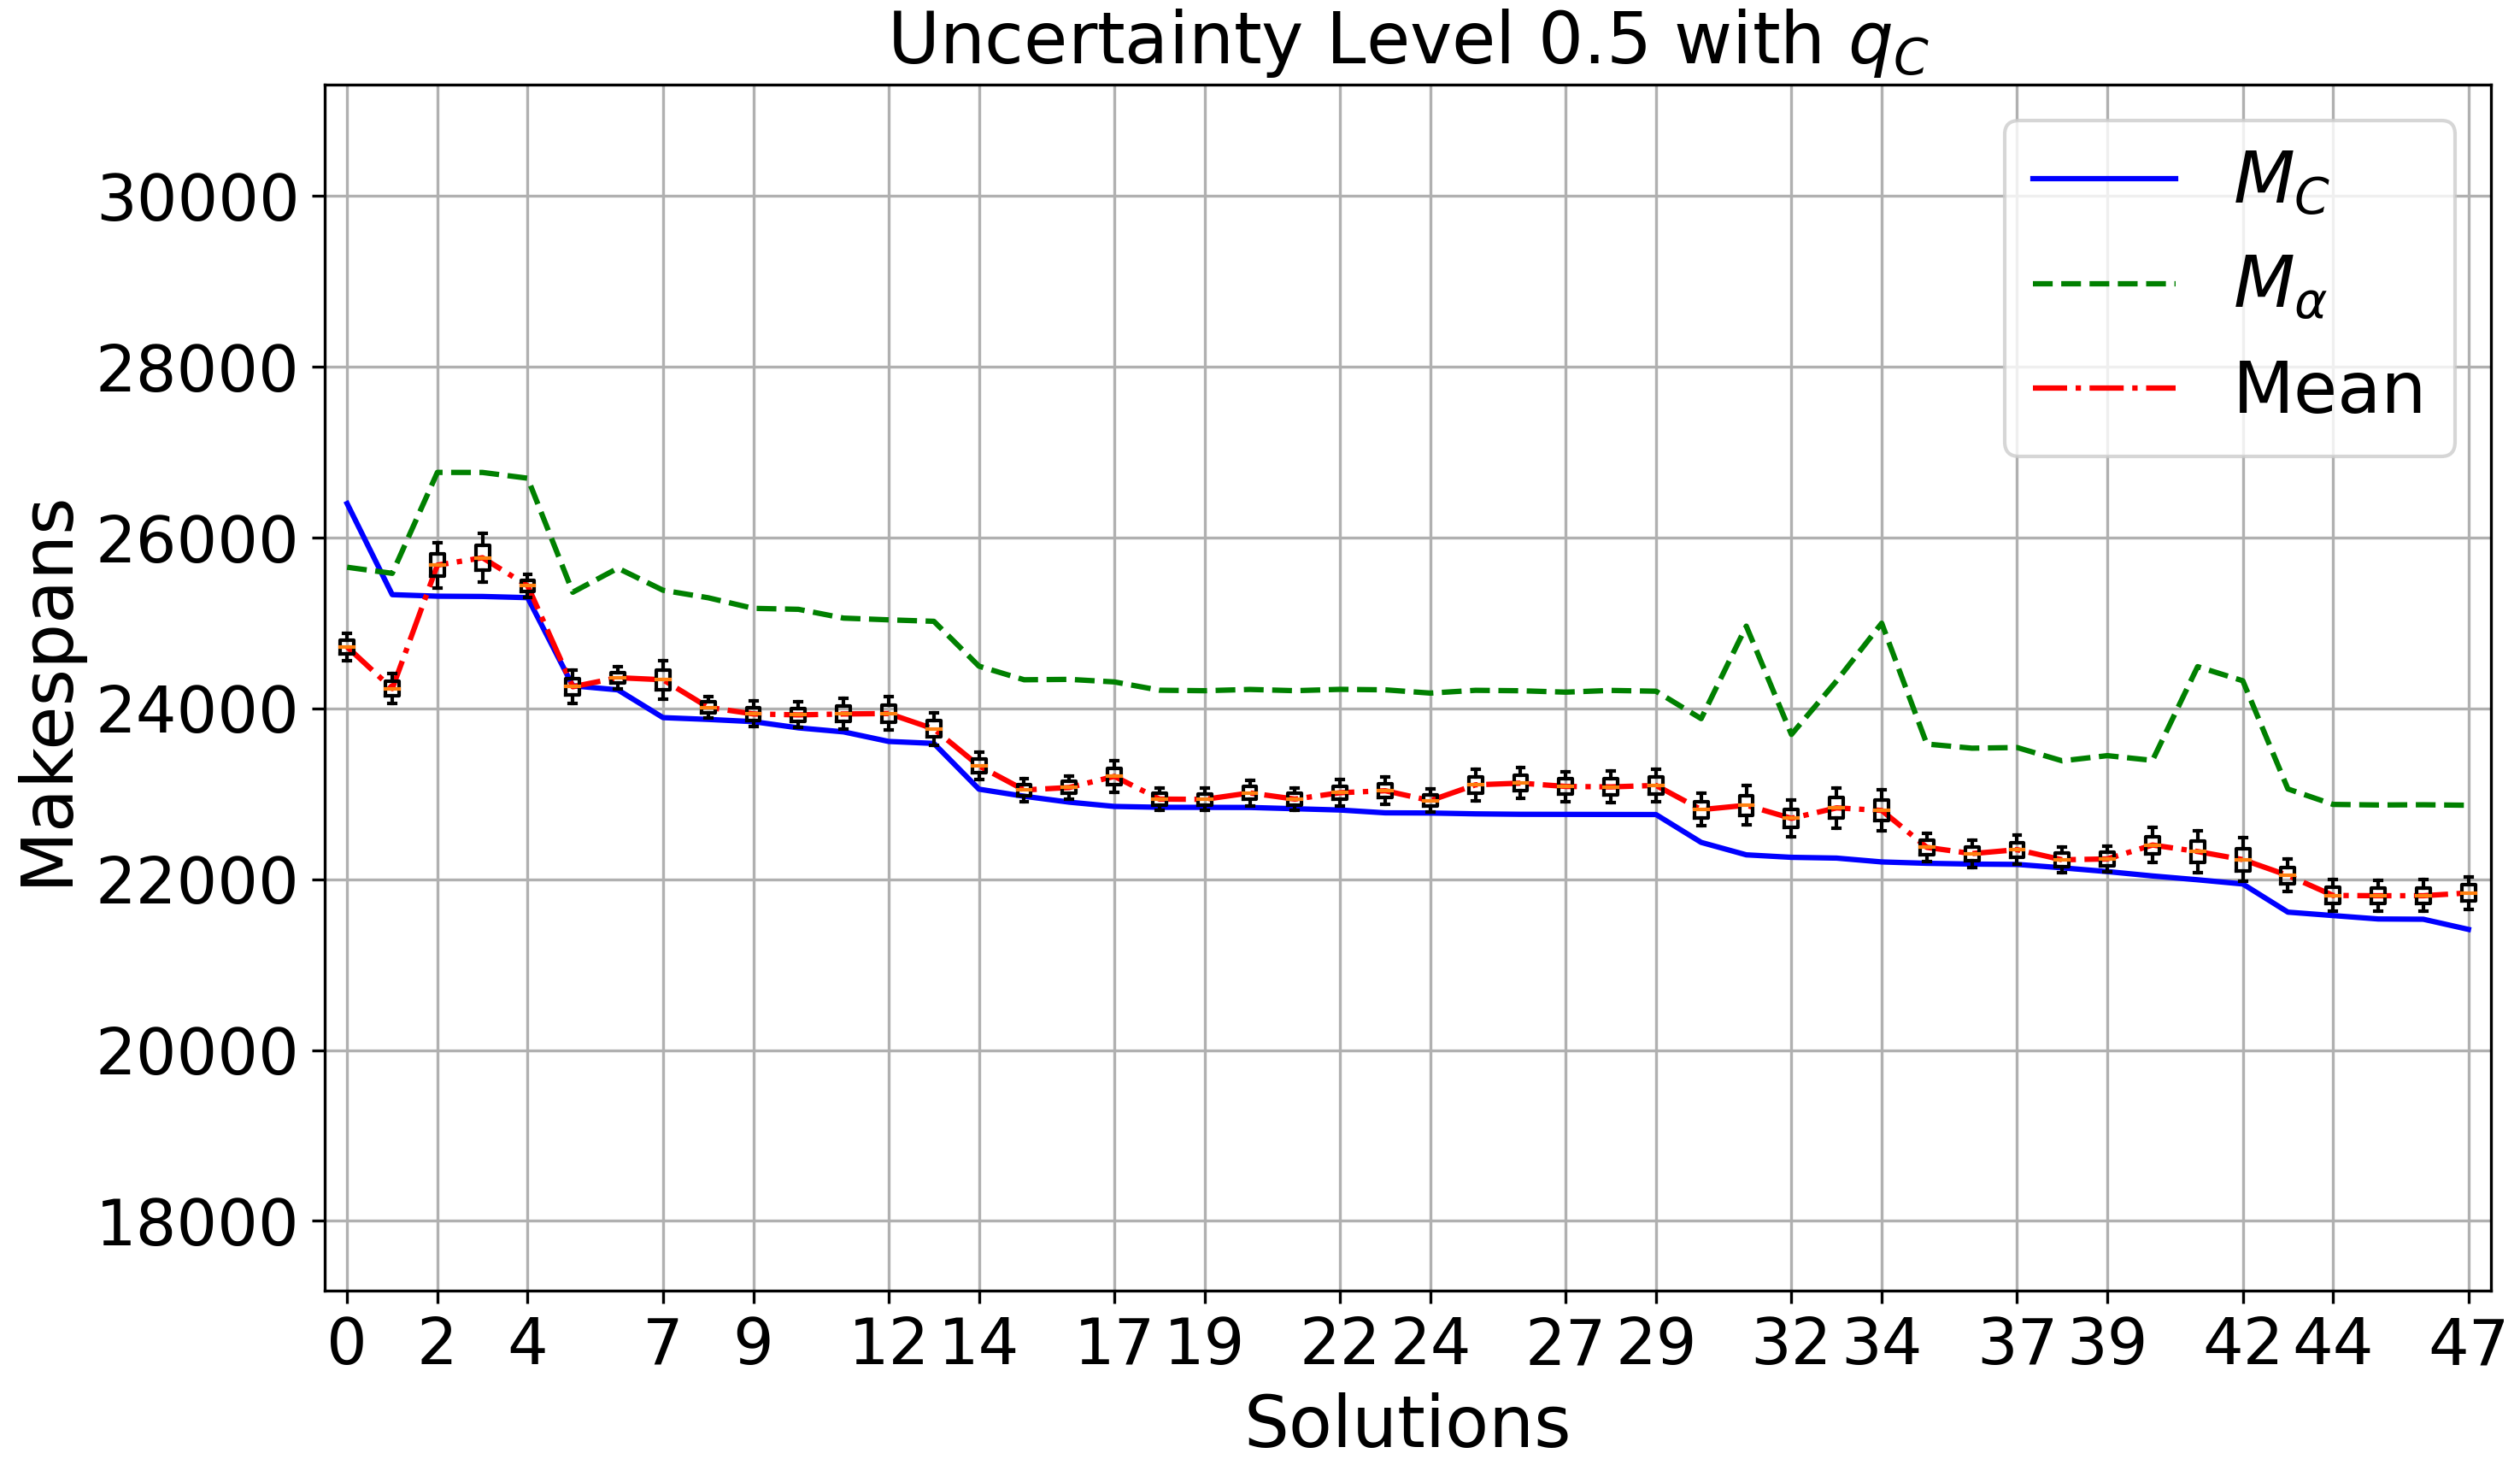
\includegraphics[width=0.47\textwidth]{images/uncertainty_caledars_2.png} }}%
    \caption{Comparison of all $M_C$ solutions returned by the CP solver, along with their corresponding $M_{\alpha}$ values and the \emph{Mean} computed over 1,000 simulations, for the synthetic \act{medium} problem with calendars and with an uncertainty level of $0.5$.}%
    \label{fig:comparison_qU_qC}%
\end{figure*}
 
In this section, we first outline the experimental settings, followed by a detailed description of the synthetic and real-world datasets used in our evaluation framework and their results. For synthetic experiments, we do not introduce other competitive methods, as the aim of these experiments is to test our framework under different uncertainty levels, problem sizes, and the presence or absence of resource calendars. For the real-world dataset, we do not compare our approach with other works due to their limitations, such as the absence of planned resource unavailability, the inability to account for uncertainty in activity durations, or scalability issues with large BPSP problems (see Section~\ref{sec:related}), which would lead to unfair comparisons.

\subsection{Experimental Setting}

\paragraph{Success Metrics} To assess the effectiveness of the proposed approach, we use two different metrics: the Normalized Probabilistic Makespan ($NPM$) and the Percentage of Improvement ($PI$). The $NPM$ evaluates the ratio between the minimum probabilistic Makespan ($M^*_{\alpha}$) and the minimum deterministic Makespan ($M^*_{C}$) obtained on synthetic experiments. It is computed as $NPM = M^*_{\alpha}/{M^*_{\text{C}}}$.

For the real-world dataset, we compute the $PI$ metric to measure the improvement between the $M^*_{\alpha}$ obtained from the optimized schedule and $M_{\text{act}}$ obtained from the actual schedule. It is calculated as $PI = ((M^*_{\alpha} - M_{\text{act}})/M_{\text{act}}) \times 100$.

\paragraph{Experimental Procedure} To transform the BPSP problems into deterministic ones, we need to define the $q$ value for each of them.
Instead of using $q_U$, we leverage the Monte Carlo simulation to obtain a more accurate estimation of the critical path compared to the one provided in the $q_U$ definition \eqref{eq:qU}.
%to the one used in 
To do that we employ \rims~\cite{MeneghelloFGR25}, a state-of-the-art business process simulator capable to accurately represent the complexity of business processes.
Specifically, we simulate the BPSP problem $1,000$ times using stochastic activity durations and identify the maximum critical path, $\pi$.
In this way, we obtain a deterministic Makespan that is closer to the probabilistic one, as we will show in Figure~\ref{fig:comparison_qU_qC}. This higher correlation between deterministic and stochastic Makespan allows us to accelerate the convergence to the minimal probabilistic Makespan $M_\alpha^*$.\footnote{In the repository \url{https://github.com/francescameneghello/IJCAI2025-Proactive-DataDriven-Scheduling-Business-Process} provides further evidence of the differences between applying $q_U$ and $q_C$. The latter allows finding $M^*_{\alpha}$ closer to $M^*_{\text{C}}$ and, within the same solver time limit, achieves a smaller $M^*_{\alpha}$ with fewer solutions, as shown in Figure~\ref{fig:comparison_qU_qC}. The downside is that using $q_C$, we cannot guarantee the lower bound property proved in Proposition~\ref{prop:lower}. }
%Instead of using $q_U$, which can be challenging to estimate due to the difficulty of determining the number of uncertain activities in the critical path---especially in BPSP problems that exhibit variability in case length and the number of resources involved---we estimate $q$ differently. Specifically, we simulate the BPSP problem $1,000$ times using stochastic activity durations and identify the maximum critical path, $\pi$. In this way, we can identify a deterministic Makespan closer to the probabilistic one as shown in Figure~\ref{fig:comparison_qU_qC}.\footnote{Our supplementary material provides further evidence of the differences between applying $q_U$ and $q_C$. The latter is not always a lower bound, but allows finding $M^*_{\alpha}$ closer to $M^*_{\text{C}}$.} 
The $q_C$ is then defined as follows~(\cite{beck2007proactive})
\[
q_C = \frac{\Phi^{-1}(1-\alpha)}{\sqrt{|\pi|}}\frac{\sqrt{Mean\{\sigma^2_{i,j}: A_i \in \pi\}}}{Mean\{\sigma^2_{i,j}: A_i \in \pi\}},
\] where $|\pi|$ is the number of activities in $\pi$.

%To retrieve $q_C$ and evaluate the solution, we use \rims~\cite{meneghello2023rimstool}, a state-of-the-art business process simulator capable of integrating predictive models to accurately represent the complexity of business processes.


After collecting all the solutions returned by the solver, we select the top $k$-solutions to be evaluated with \rims. These $k$-solutions are identified based on the last significant improvement\footnote{A significant improvement in the ordered list of deterministic solutions is defined as a $\Delta_i = (M_{\text{C}, j} - M_{\text{C}, i})/M_{\text{C}, j} \geq 0.20$ where solution $j$ precedes solution $i$.}, which tends to remain consistent in subsequent solutions. For instance, in Figure~\ref{fig:calendar_qC}, the last significant improvement is observed between solutions $42$ and $43$, marked by a notable step on the $M_{\text{C}}$ line, followed by a plateau. %extending until solution $47$. 

A 3-minute time limit is set for the CP solver, and the evaluation with \rims, thanks to the $k$-solution selection, takes an average of 5 minutes, with a maximum of 15 minutes for the largest problem in the DayHospital experiment. The experiments are conducted on a PC with 16 GB of RAM and an M2 processor.

\subsection{Synthetic Data Experiment} 

\paragraph{The Data} As synthetic data we use three problems from a set of publicly available JSP beanchmarks of different size \act{small} ($10 \times 10$), \act{medium} ($20 \times 20$), \act{big} ($50 \times 20$)~\cite{beanchmarks}\footnote{In the repository \url{https://github.com/francescameneghello/IJCAI2025-Proactive-DataDriven-Scheduling-Business-Process}, three other problems of different sizes are reported.}, where with $10 \times 10$ we indicate a problem with $10$ cases with $10$ activities for each case. For each of the problems, we set three levels of uncertainty $u \in \{0.1, 0.5, 1\}$ to define the standard deviation of each activity $a_{i,j}$ as a random number within the interval $\sigma_{i,j}= [0, u*\mu_{i,j}]$.
For each resource involved, we generate the corresponding calendars, assuming a working week of 5 days and 8 hours per day.

%Furthermore, we extend the synthetic data by generating three additional problems with the same structure, but activity durations depend on the type of case. The types represent three possible categories of patients in a hospital: the rare \act{red}, which leads to increased activity durations; \act{white}, which results in durations closer to the mean; and finally \act{yellow}, which falls in between the two.

\paragraph{Results} Table~\ref{tab:results_synthetic} presents the normalized probabilistic Makespans ($NPM$), showing that in the first set of experiments, the presence or absence of calendars does not significantly impact performance, except for the \act{Big} size at uncertainty levels $0.1$ and $1.0$. 
From an empirical analysis of the experiments with the presence of resource calendars, we note that a $q_C$ with respect to $q_U$ allows for representing activity durations closer to real times, enabling it to effectively leverage the planned availability and unavailability of resources to optimize the schedule.
Figure~\ref{fig:calendar_qC} shows that the average Makespans overlap with $M_C$, and $M_\alpha$ is slightly higher.  In contrast, $q_U$, as shown in Figure~\ref{fig:calendar_qU}, guarantees the lower bound (Section~\ref{sec:stoc_to_det}), but results in a worse solution compared to $q_C$.
Variance in $q$ may lead to a significant difference between the deterministic and the corresponding probabilistically minimal Makespans, even if their correlation remains. 
%This behavior appears more evident in the second set of experiments (see dark lines of Table~\ref{tab:results_synthetic}) where the $NPM$ metrics with calendars are always close to $1$ or slightly below. 


\subsection{DayHospital Experiment} 

\paragraph{The Data} In this experiment, we apply our approach to a real-world BPSP problem. Specifically, we use an entire year (2021) of data from DayHospital to learn the BPSP parameters and minimize the Makespan for the subsequent five months (January-May 2022), which serve as the test set.
The event log includes timestamped activities along with their designated resources as shown in Table~\ref{table:real_log_DT}. This allows us to identify the activities, the precedence relationships, and the resources, including their capacities and calendars, to define the BPSP problem.
Between 50 and 1,000 patients are treated every day in the hospital, depending on whether it is a weekday or a weekend, with over 1,600 activities taking place on the busiest days. 
To properly evaluate our approach, we compare the Makespan given from the simulation of the actual schedule and the $M^*_{\alpha}$ found with our approach.



\paragraph{Results}
Table~\ref{tab:results_hospital} reports the results achieved on the hospital dataset. We divided the days into \act{small}, \act{medium}, and \act{big} categories based on the number of activities treated in a day. For \act{medium} and \act{big} days, we observe, on average, a significant reduction in the global Makespan, up to 14\%, which corresponds to a reduction of approximately 4 hours. In the case of \act{small}, the scope for improvement is limited, yet we still observe improvements, even if at a slightly lower percentage. 




\begin{table}[tb]
    \centering
    \resizebox{.80\columnwidth}{!}{
    \begin{tabular}{c|cc|cc|cc}
        \toprule
        \textbf{Un. Level} & 0.1 & 0.1 & 0.5 & 0.5 & 1 & 1 \\
        \midrule
        \textbf{Calendar} & x & \checkmark & x & \checkmark & x & \checkmark \\
        \midrule \midrule
        \act{Small} &  1.00  &  1.00 & 1.03 & 1.00 & 1.13 & 1.13 \\
        \midrule
        \act{Medium} &  0.99  &  1.00 & 1.03 & 1.00 & 1.10 & 1.10 \\
        \midrule
        \act{Big} &  1.09  &  1.00 & 1.07 & 1.07 & 1.12 & 1.18 \\
        \bottomrule
    \end{tabular}
    }
    \caption{The NPM metrics are presented for each size, with and without the resource calendars.}
\label{tab:results_synthetic}
\end{table}


\begin{table}[tb]
    \centering
    \resizebox{.99\columnwidth}{!}{
    \begin{tabular}{l@{\hskip 0.05in}c@{\hskip 0.05in}c@{\hskip 0.05in}c@{\hskip 0.05in}c@{\hskip 0.05in}c@{\hskip 0.05in}c@{\hskip 0.05in}}
        \toprule
        \multirow{2}{*}{\textbf{Days}} & \textbf{Av.} & \textbf{Av. } & \textbf{Av.} & \textbf{Av.} & \textbf{Max} & \textbf{Av.} \\
         & \textbf{\#Cases} & \textbf{ \#Activities} & \textbf{ \#Resources} & \textbf{\% Imp.} & \textbf{\% Imp.} & \textbf{Imp.} \\
        \midrule
        \act{Small} &  98 &  136 & 33 & -1.2\% & -6\% & -14min \\
        \midrule
        \act{Medium} &  717  & 1242 & 237 & -4.8\% & -12\%& -69min \\
        \midrule
        \act{Big} &  848  & 1505 & 266  & -5.9\% & -14\% & -87min \\
        \bottomrule
    \end{tabular}
    }
    \caption{The days are divided into 3 groups based on 33rd and 67th percentiles.}
\label{tab:results_hospital}
\end{table}


